
\section{Introduction}



\IEEEPARstart
As the cornerstone of autonomous and intelligent driving systems, perception enables vehicles to comprehend the driving environment and support safe decision-making. Nevertheless, onboard sensors are limited in range and coverage, resulting in incomplete, uncertain, or degraded environmental understanding in complex scenarios~\cite{zhang2023perception}. Vehicle-to-Everything (V2X)~\cite{chen2023cellular}-enabled cooperative perception (CP) overcomes these constraints through multi-agent collaboration, extending perceptual horizons beyond line-of-sight limitations and occlusion. By synergizing vehicle-to-vehicle (V2V) and vehicle-to-infrastructure (V2I) communications~\cite{tian2024msra}, CP demonstrates significant advantages in occlusion-rich environments and long-range perception tasks, and emerges as a pivotal technological approach for safety-enhanced driving systems~\cite{yang2024v2x,jiang2024weather,xiang2022v2xp}.

%{W}{ith} the rapid development of intelligent transportation technologies, intelligent driving systems are increasingly regarded as a cornerstone for achieving safe, efficient and intelligent traffic management. Among their core components, perception provides essential information for path planning, motion control, and decision-making. However, single-vehicle perception systems rely solely on onboard sensors, whose limited sensing range cannot fully capture the surrounding environment. This leads to perception blind spots, while long-range object detection accuracy quickly degrades in complex and dynamic scenarios, making it difficult to meet the stringent requirements of intelligent driving for accuracy and robustness~\cite{zhang2023perception}.

%The emergence of Vehicle-to-Everything (V2X) technologies offers a promising pathway to overcome these limitations. Through vehicle-to-vehicle (V2V) and vehicle-to-infrastructure (V2I) communications, cooperative perception (CP) can effectively alleviate the shortcomings of single-vehicle perception in terms of coverage and recognition accuracy, and has demonstrated significant advantages in scenarios involving occlusion, long-range perception, and challenging interactions~\cite{yang2024v2x,jiang2024weather,xiang2022v2xp}. Consequently, cooperative perception has become a critical technology for realizing safe and efficient intelligent driving.



Despite its theoretical potential to extend environmental awareness, the practical implementation of CP still faces critical safety challenges. These challenges primarily originate from inherent communication and computation latencies. Communication latency causes environmental representation lag—vehicles receive perception data that typically reflects historical states. Simultaneously, computation latency during multi-source data fusion further exacerbates this issue, delaying perception result updates. As illustrated in Figure~\ref{fig_1}, the temporal discrepancy leads to risk assessment inaccuracies: a vehicle incorrectly identified as collision-free in real-time may execute erroneous decisions due to lagged perception results. These perception-reality gaps from dual-latency directly elevate collision risks, particularly in occlusion scenarios where temporal inconsistency masks the threat trajectories~\cite{shenkut2024impact,wang2024current}. Through dual-latency compensated CP (Figure~\ref{fig_1}), temporal consistency between perception result and the physical world is restored, yielding more accurate and timely perception and thereby reducing safety risks.

%Despite the significant potential of CP to enhance sensing performance, its practical deployment still faces critical challenges. Among these, communication and computation latencies have emerged as major bottlenecks restricting real-time responsiveness and reliability. In V2V cooperation, perception data must be exchanged frequently among vehicles, which unavoidably results in communication latency. Furthermore, CP involves computationally intensive tasks such as multi-sensor fusion within a single vehicle, multi-vehicle perception data fusion, and object detection, all of which contribute to non-negligible computation latency. The combined impact of communication and computation latencies can cause perception outputs to fail to keep pace with highly dynamic traffic environments(as shown in Figure~\ref{fig_1}), thereby degrading control efficiency and compromising decision-making safety~\cite{shenkut2024impact,wang2024current}.


%Existing research has explored several strategies to mitigate the impact of communication latency in cooperative perception. One common approach is to reduce communication load by decreasing the volume of transmitted data, such as through data compression or region-of-interest selection. While this method effectively reduces bandwidth usage, latency inevitably persists and cannot be fully eliminated. Another line of work focuses on data alignment, where the receiver aligns its local perception with the incoming perception data to minimize the effects of latency. However, such approaches may introduce temporal inaccuracies and information distortion, potentially compromising safety. More recently, prediction-based compensation has been proposed, in which the receiver employs predictive models to estimate the current state based on limited historical data. Although this method shows promise, it still suffers from several limitations: (i) insufficient historical data when perception information is first received, leading to reduced prediction accuracy; (ii) lack of model adaptability, as most existing approaches adopt generic prediction models that cannot be tailored to the characteristics of individual vehicles; and (iii) computational burden, since receivers in multi-vehicle systems must perform separate prediction compensation for each transmitting vehicle due to heterogeneous latencies, thereby increasing computational cost and undermining real-time performance.
%To address the aforementioned challenges, prior studies have attempted to reduce communication latency or mitigate its impact through various strategies. For example, some approaches compress perception data~\cite{xu2022opv2v,wang2023vimi,zheng2024real}, select regions of interest~\cite{yuan2022keypoints,lohdefink2020focussing,hu2022where2comm}, or restrict communication links to reduce communication overhead~\cite{liu2020who2com,qu2024model}. While such methods effectively reduce communication overhead, they cannot eliminate latency, and communication latency still degrade perception performance. To address this, some studies align perception information received to the receiver’s local perception, thereby synchronizing the transmitted data with the receiver’s temporal framework~\cite{liu2024select2col,liu2024v2x,lin2024v2vformer,lei2024robust,bai2023vinet}. However, this strategy risks propagating abnormal information, potentially introducing serious safety risks. Other studies~\cite{wang2025cmp,rossle2024unlocking,fang2024pacp,yu2023vehicle,lei2022latency} employ generic prediction models on the receiver vehicle, using limited historical data to compensate for communication latency. However, such methods may fail during the initial transmission of a vehicle, when no useful historical data is available. In addition, generic models lack personalization and cannot adapt to the unique driving patterns and perception characteristics of different vehicles. To overcome these limitations, a vehicle-specific prediction model, which leverages the full historical perception data of the transmitting vehicle to model its driving habits and provide more accurate predictions, is proposed.

Existing studies mitigate communication latency by reducing data load (e.g., compression~\cite{xu2022opv2v,wang2023vimi,zheng2024real}, ROI selection~\cite{yuan2022keypoints,lohdefink2020focussing,hu2022where2comm} or restricting communication links~\cite{liu2020who2com,qu2024model}), which alleviate communication overhead but cannot eliminate delay. Moreover, data alignment approaches~\cite{liu2024select2col,liu2024v2x,lin2024v2vformer,lei2024robust,bai2023vinet} fuse local and received perception to mitigate latency. Nonetheless, they may introduce temporal errors, information distortion, and even abnormal information, thereby posing potential safety risks. Furthermore, prediction-based compensation methods~\cite{wang2025cmp,rossle2024unlocking,fang2024pacp,yu2023vehicle,lei2022latency}, typically deployed on the receiving vehicle, is regarded as an effective solution to improve timeliness. However, it still suffers from several challenges: insufficient historical data at the initial reception stage, limited adaptability of generic models to heterogeneous vehicle characteristics, and heavy computational overhead when compensating heterogeneous delays in multi-vehicle systems. 

For computation latency, most existing approaches focus on resource scheduling optimization~\cite{xu2024intelligent,lu2025joint} or hardware acceleration~\cite{fan2023hardware} to shorten processing time. Although these solutions can partially alleviate processing delays, they fail to resolve the problem of outdated perception results, which are caused by computation latency. 

Based on the above studies, although prediction-based compensation methods represent an effective strategy to address latency, its deployment on the receiving side suffers from data scarcity, limited accuracy, and heavy computational burden, while existing methods targeting
computation-latency fail to resolve the fundamental issue of outdated perception. To overcome these limitations, this paper proposes Dual-Latency Prediction Compensation Mechanism (DLPCM) based on a Vehicle-Specific Prediction Model (VSPM) with Model State Transmission (MST), which jointly compensates for both communication and computation latencies. By shifting the prediction model to the sending side, the sender can leverage abundant historical data to achieve accurate, vehicle-specific prediction while avoiding data insufficiency at the receiver. Moreover, instead of transmitting raw perception data, compressed intermediate model states are sent, which offloads redundant computation, reduces communication overhead, and ensures sufficient historical context. This design ultimately enables joint compensation of communication and computation latency, thereby improving system real-time performance, robustness, and reliability.

%Although this shift introduces new challenges such as model transmission, these challenges highlight the research value and innovation of the proposed solution.

%To overcome these limitations, we propose a dual-latency prediction compensation mechanism based on a vehicle-specific prediction model, which jointly compensates for both communication and computation latencies. At the transmitting side, a lightweight temporal prediction model is deployed and trained using the vehicle’s historical perception data. During the initial exchange, only the model parameters are transmitted; in subsequent cycles, compressed intermediate model states are sent instead of raw perception data. At the receiver side, the transmitted states and the received prediction model are combined to reconstruct the transmitter’s future perception data by jointly compensating communication and computation latencies. Meanwhile, the receiver leverages its own latest local perception to compensate for residual computation latency. Finally, all compensated perceptions are synchronized to the expected result time $t_{result}$ and fused, producing a timely cooperative perception output.  

%This design offers several advantages from multiple perspectives:  (i) The prediction model is trained on each vehicle’s own historical perception data, enabling it to capture personalized motion patterns and perception characteristics that generic models cannot. Moreover, accurate prediction requires sufficient historical input, which is naturally guaranteed by placing the model at the transmitting vehicle, where the complete historical perceptions are available. This design ensures both higher prediction accuracy and robustness compared with approaches that rely on limited history. (ii) Intermediate state transmission enables a more efficient allocation of computational resources. Without this design, each receiving vehicle would redundantly perform the entire prediction process, even though much of the computation overlaps. By contrast, offloading the majority of the prediction process to the transmitter eliminates redundant computation, while receivers only perform the necessary residual prediction compensation tailored to their different latency conditions.  (iii) Intermediate states inherently encode long-term history, providing robust support for prediction even when a vehicle communicates for the first time or lacks sufficient historical information. At the same time, these states are far smaller than raw historical perceptions, and even when compared to a single perception frame, the compressed states substantially reduce communication load.  (iv) By explicitly compensating for both communication and computation latencies at the receiver, the proposed mechanism enhances the timeliness and stability of cooperative perception. (v) Since the proposed mechanism provides latency-compensation and temporally aligned perception results, it can be flexibly integrated with different cooperative perception fusion frameworks, offering strong adaptability across varying system designs.

\begin{figure*}[!t]
\centering
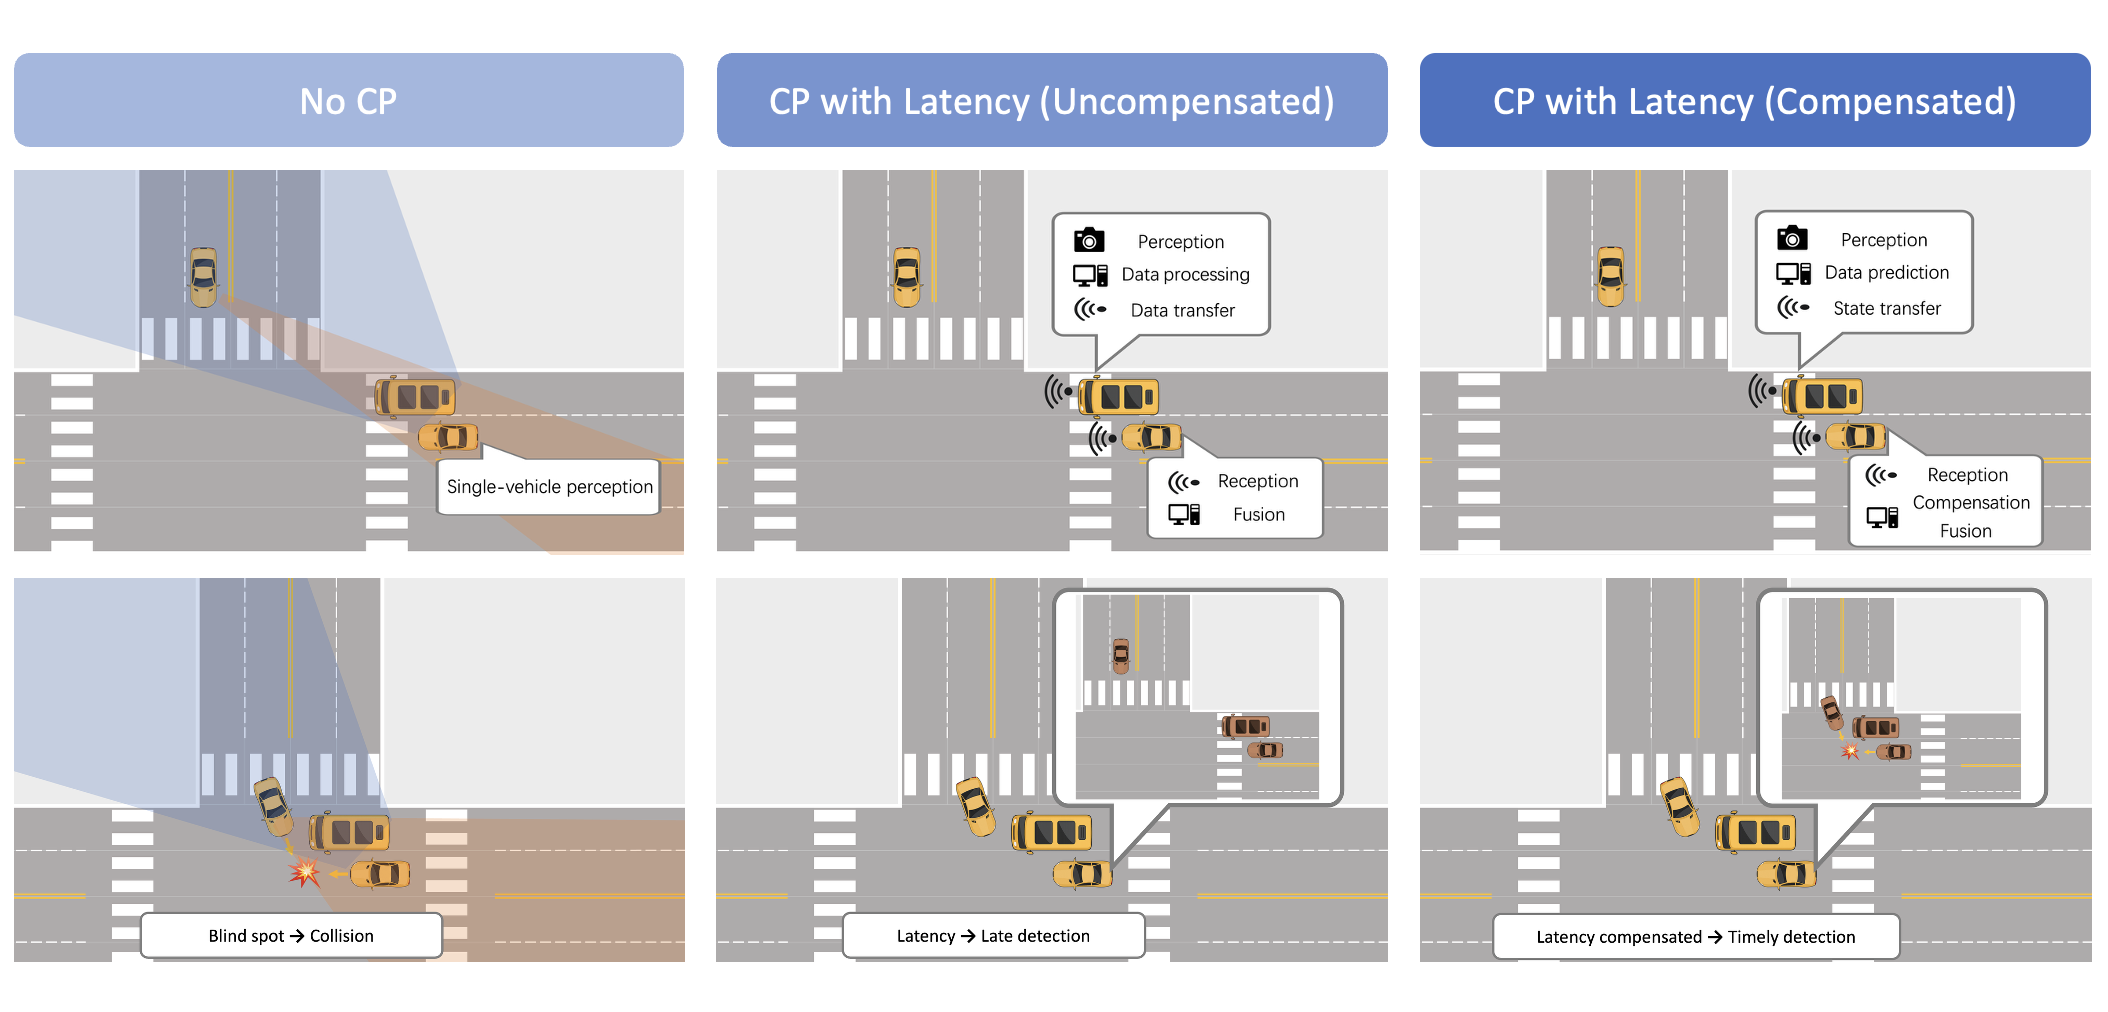
\includegraphics[width=7in]{figure1.jpg}
\caption{\textbf{Example of vehicle perception results under dual-latency.} The figure illustrates three scenarios: \textbf{No CP}, where a single vehicle relies solely on its onboard sensors, resulting in blind spots and potential collisions; \textbf{CP with latency (Uncompensated)}, where cooperative perception is performed but communication and computation latencies cause late detection; and \textbf{CP with latency (Compensated)}, where the proposed mechanism integrates prediction and latency compensation, enabling timely detection and improved real-time performance of perception.
}
\label{fig_1}
\end{figure*}

The main contributions of this paper are summarized as follows:

\begin{enumerate}

\item{Dual-Latency Prediction Compensation Mechanism: We propose a novel compensation mechanism that jointly addresses both communication and computation latencies, ensuring timely and reliable cooperative perception in dynamic traffic environments.}

\item{Vehicle-Specific Prediction Model: Instead of relying on generic models, we design a lightweight prediction model trained on each vehicle’s historical perception data, which enables personalized and more accurate prediction while enhancing robustness against diverse motion patterns.}

\item{Model State Transmission: We introduce an efficient communication strategy that transmits compressed intermediate model states rather than raw perception data. This design not only reduces communication overhead but also offloads redundant computation from the receiver, ensuring efficient resource utilization and sufficient historical context for accurate prediction.}

\item{Enhanced System Performance: By combining personalized prediction, efficient model state transmission, and dual-latency compensation, the proposed mechanism significantly improves the real-time performance, robustness, and adaptability of cooperative perception. Experiments on V2X-Sim and complementary DAIR-V2X-C official detection/BEV forecasting evaluations further validate its effectiveness under simulated and real cooperative driving scenarios.}
\end{enumerate}

\noindent


This paper is organized as follows: Section 2 reviews related work and research background; Section 3 introduces in detail the dual-latency prediction compensation mechanism based on the vehicle-specific Prediction Model proposed in this paper; Section 4 provides experimental setup and result analysis; finally, Section 5 summarizes the paper and looks forward to future research directions.
